\section{Experiments}

\subsection{Setup}

We test on synthetic ($N{=}5{,}000$, $K \in \{2, 4\}$, controlled $\Delta\tau$ and $\Delta\pi$, 100 Monte Carlo (MC) runs) and semi-synthetic data-generating processes (DGPs) spanning four NLP tasks: sentiment analysis (TweetEval~\cite{barbieri2020tweeteval}, $K{=}4$), hate speech detection (CivilComments, $K{=}4$), stance detection ($K{=}5$; Appendix~\ref{app:stance}), and topic classification (AG News, $K{=}4$; Appendix~\ref{app:agnews}), with full specifications in Appendix~\ref{app:dgp}.

We compare: (1) \textit{Naive} (no correction), (2) \textit{Global} (pooled confusion matrix, equivalent to PPI/DSL~\cite{angelopoulos2023ppi,egami2023dsl} with homogeneous error), (3) \textit{Stratified MLE} (per-subgroup DSL without shrinkage), (4) \textit{HB EC-HTE} (per-subgroup correction), (5) \textit{PPCI}~\cite{sui2026ppci}, and (6) \textit{EC-HTE+PPCI}.
For CausalForest~\cite{wager2018causal}, we compare naive, global, and EC-HTE variants.
Primary metrics are $|\text{bias}|$, root mean squared error (RMSE), and 95\% confidence interval (CI) coverage, averaged across subgroups and 100 MC runs.
Robustness validations cover eight conditions including asymmetric errors, subgroup misspecification, and treatment-dependent misclassification (all $\geq$89.5\% coverage; Appendices~\ref{app:hatespeech}--\ref{app:treatment_dep}).
Semi-synthetic evaluation uses empirical confusion matrices from nine LLMs (five proprietary, four open-source) across two datasets (Appendix~\ref{app:realcm_bias}; semi-real CM validation in Appendix~\ref{app:semireal}; open-source LLM validation in Appendix~\ref{app:multilm_opensource}).

\subsection{Empirical Validation of the Bias Identity}
\label{sec:bias_mechanism}

\begin{table}[t]
\centering
\caption{Results under moderate heterogeneity and semi-synthetic data. Moderate: $\Delta\pi \leq 0.10$; TweetEval: empirical subgroup structure ($K{=}4$). Metrics averaged over subgroups, $z$-levels, 100 MC runs. $^\dagger$RMSE exceeds Global.}
\label{tab:main_supp}
\small
\resizebox{\columnwidth}{!}{%
\begin{tabular}{ll ccc}
\toprule
Configuration & Method & $|\text{Bias}|$ & RMSE & Cov. \\
\midrule
\multirow{4}{*}{\shortstack[l]{Synthetic DIM\\$K{=}2$, moderate, $n{=}250$}}
 & Naive & 0.018 & 0.064 & 0.95 \\
 & Global & 0.009 & 0.074 & 0.96 \\
 & Strat.\ MLE & \textbf{0.005} & 0.075$^\dagger$ & 0.97 \\
 & HB EC-HTE & \textbf{0.005} & 0.075$^\dagger$ & 0.97 \\
\midrule
\multirow{4}{*}{\shortstack[l]{Semi-synthetic\\TweetEval, extreme, $n{=}250$}}
 & Naive & 0.027 & 0.103 & 0.93 \\
 & Global & \textbf{0.023} & 0.124 & 0.92 \\
 & Strat.\ MLE & 0.032 & 0.248$^\dagger$ & 0.91 \\
 & HB EC-HTE & 0.027 & 0.225$^\dagger$ & 0.91 \\
\bottomrule
\end{tabular}}
\end{table}

We verify Theorem~\ref{thm:bias_identity} on a $K{=}2$ grid (520 configurations, $\Delta\pi \in [0, 0.25]$, $\Delta\tau \in (0, 0.50]$) and a $K{=}4$ grid (Appendix~\ref{app:dgp}).
Regressing observed subgroup bias on $\delta_s \cdot \Delta\tau / (1{-}2\bar{\pi})$ yields $R^2 = 0.994$ ($K{=}2$) and $0.97$ ($K{=}4$); residual variance reflects MC noise ($R^2 \geq 0.976$ even at $P(Z{=}1) = 0.1$; Appendix~\ref{app:classimbalance}).
Global correction worsens bias in 50\% of $K{=}2$ configurations (260/520, excluding $\Delta\pi{=}0$), with amplification reaching 2.86$\times$ ($K{=}2$) and 2.41$\times$ ($K{=}4$); Figure~\ref{fig:heatmap} visualizes the amplification surface.
Global correction also reverses the sign of estimated CATE in 14.9\% of configurations at $\tau(0) = 0.03$, rising to 31\% at $\tau(0) = 0.01$ (Figure~\ref{fig:sign_reversal_rate}), with all nine real LLMs amplifying bias; EC-HTE eliminates sign reversal (Figure~\ref{fig:sign_reversal}; Appendix~\ref{app:policy_reversal}).
Cross-task validation on stance detection ($K{=}5$, Appendix~\ref{app:stance}) confirms sign reversal (13.3\% $\to$ 3.3\%) and reveals limitations when $\mathrm{FNR} > 0.50$.

\paragraph{Real-world case study.}
On the UC Berkeley Hate Speech corpus (Appendix~\ref{app:hatespeech}), GPT-4.1 per-subgroup misclassification rates range from 0.266 to 0.383 ($\Delta\pi = 0.117$), confirming that subgroup-heterogeneous error arises in real annotation settings.
At $\mathrm{FNR} = 53.3\%$, however, the CM approaches singularity, confirming the boundary condition: EC-HTE needs both sufficient labels \emph{and} $\mathrm{FNR} < 0.50$.
On CivilComments~\cite{borkan2019nuanced} (Appendix~\ref{app:civilcomments}), all three tested LLMs exhibit $\Delta\pi > 0.05$ across text-feature subgroups, with the largest heterogeneity $\Delta\pi = 0.184$ (GPT-4o FPR).

\begin{figure}[t]
\centering
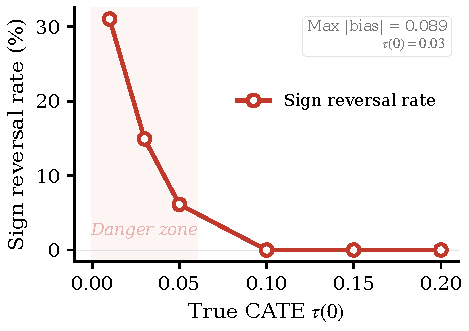
\includegraphics[width=\columnwidth]{figures/fig_sign_reversal_C.pdf}
\caption{Sign reversal rate increases as true CATE $\tau(0) \to 0$: at $\tau(0) = 0.03$, 14.9\% of configurations exhibit sign reversal; all nine real LLMs amplify bias; EC-HTE eliminates reversal in the $K{=}2$ setting.}
\label{fig:sign_reversal_rate}
\end{figure}

\subsection{Correction Evaluation}
\label{sec:ec_hte_eval}

Table~\ref{tab:main_results} presents the main results.
In the $K{=}2$ extreme row, global correction \emph{increases} $|\text{bias}|$ relative to naive (0.059 vs.\ 0.058), confirming Theorem~\ref{thm:bias_identity}; F-L corrections fare worse (0.122--0.168).
HB EC-HTE reduces $|\text{bias}|$ from 0.059 to 0.008 (7.4$\times$); relative to stratified MLE (0.012), the advantage is 1.5$\times$ with lower RMSE from partial pooling. At $K{=}4$, bias reduces from 0.056 to 0.012 (4.7$\times$), maintaining near-nominal coverage (0.94--0.96).
Under moderate heterogeneity ($\Delta\pi \leq 0.10$), methods converge: HB EC-HTE and global correction yield indistinguishable $|\text{bias}|$ (0.005 vs.\ 0.009) and RMSE (0.075 vs.\ 0.074), confirming the diagnostic's guidance (Table~\ref{tab:main_supp}).
On semi-synthetic TweetEval ($K{=}4$, empirical subgroup structure), EC-HTE RMSE (0.225) exceeds global (0.124) because the empirical $\Delta\pi$ (${\approx}0.10$) falls below the recommended threshold; practitioners who apply the screening criterion correctly would retain global correction here (Table~\ref{tab:main_supp}).
EC-HTE requires $n_{\text{expert}} \geq 250$ ($K{=}2$) or $\geq 500$ ($K{=}4$); below this, RMSE exceeds global (Figure~\ref{fig:budget_compact}).
At $K{=}8$ with $n_{\text{expert}}{=}250$ (${\approx}31$ labels per subgroup), HB partial pooling reduces stratified MLE RMSE by 47\% but still exceeds global correction, confirming $K \leq 4$ as the practical scalability boundary (Appendix~\ref{app:k8_subgroups}).

\paragraph{CausalForest.}
CausalForest~\cite{wager2018causal} with a noisy $\hat{Z}$ inherits the same $M_{\text{global}}^{-1} M_s$ structure.
EC-HTE reduces $|\text{bias}|$ from 0.191 to 0.039 (4.9$\times$) with coverage 0.90 ($K{=}4$, $n{=}500$; oracle coverage decomposition in Appendix~\ref{app:cf_oracle}); R-learner yields comparable reduction (89\%, Appendix~\ref{app:rlearner}), confirming the bias arises from the confusion matrix structure, not the downstream estimator.

\paragraph{PPCI composition.}
Under joint covariate and outcome misclassification, EC-HTE+PPCI reduces $|\text{bias}|$ from 0.179 to 0.007, with coverage $\geq$94\% (Appendix~\ref{sec:ppci}).

\begin{table}[t]
\centering
\caption{Main results (extreme heterogeneity). Metrics averaged over subgroups, $z$-levels, 100 MC runs. Bold: lowest $|\text{bias}|$. $^\dagger$RMSE exceeds Global. F-L Scalar/Per-sub.: \citet{frazis2003estimating}. Moderate and semi-synthetic results in Table~\ref{tab:main_supp}; MC SEs $\leq 0.005$ (Appendix~\ref{app:mcse}). CausalForest plug-in SE achieves 93.8\% aggregate coverage; a bootstrap procedure ($B{=}100$) recovers $\geq$95\% at all budgets (Appendix~\ref{app:bootstrap_se}).}
\label{tab:main_results}
\resizebox{\columnwidth}{!}{%
\begin{tabular}{ll ccc}
\toprule
Configuration & Method & $|\text{Bias}|$ & RMSE & 95\% CI Cov. \\
\midrule
\multirow{6}{*}{\shortstack[l]{DIM\\$K{=}2$, $n{=}250$}}
 & Naive & 0.058 & 0.090 & 0.82 \\
 & Global & 0.059 & 0.099 & 0.87 \\
 & F-L Scalar & 0.122 & 0.159 & 0.68 \\
 & F-L Per-sub. & 0.168 & 0.220 & 0.65 \\
 & Strat.\ MLE & 0.012 & 0.094 & 0.95 \\
 & HB EC-HTE & \textbf{0.008} & 0.089 & 0.94 \\
\midrule
\multirow{4}{*}{\shortstack[l]{DIM\\$K{=}4$, $n{=}500$}}
 & Naive & 0.062 & 0.113 & 0.88 \\
 & Global & 0.056 & 0.125 & 0.91 \\
 & Strat.\ MLE & \textbf{0.010} & 0.127$^\dagger$ & 0.95 \\
 & HB EC-HTE & 0.012 & 0.120 & 0.96 \\
\midrule
\multirow{3}{*}{\shortstack[l]{CausalForest\\$K{=}4$, $n{=}500$}}
 & Naive & 0.208 & 0.231 & 0.44 \\
 & Global & 0.191 & 0.244 & 0.58 \\
 & EC-HTE Forest & \textbf{0.039} & 0.224 & 0.90 \\
\bottomrule
\end{tabular}}
\end{table}

\subsection{Diagnostic and Operating Conditions}
\label{sec:diagnostic}

Proposition~\ref{prop:debiasing_hurts} provides a $\Delta\tau$-free diagnostic: global correction increases bias in subgroup $s$ iff $|\delta_s| / ((1-2\bar{\pi}) \cdot \pi_s) > 1$, computable from a pilot sample without estimating treatment effects.
The diagnostic achieves subgroup-level AUC $= 0.86$ under symmetric misclassification (Appendix~\ref{app:diagnostic_roc}) and $0.96$ under asymmetric misclassification (Appendix~\ref{app:asymmetric}); under relaxed screening, 79\% of real LLM--dataset pairs show RMSE improvement with coverage $\geq$93\% (Appendix~\ref{app:screening}).

\paragraph{Operating conditions.}
EC-HTE requires: (i)~$\Delta\pi > 0.15$, (ii)~$n_{\text{expert}} \geq 250$ for $K{=}2$, (iii)~$\mathrm{FPR}_s, \mathrm{FNR}_s < 0.50$, (iv)~$K \leq 4$, and (v)~$n_{\text{expert}} \geq 500$ under asymmetric errors; when unmet, global correction achieves lower RMSE (Appendix~\ref{app:k8_subgroups}).
These thresholds reflect a bias--variance tradeoff: the crossover point shifts with $K$ and expert budget (Figure~\ref{fig:budget_compact}).
Across 11 real LLM--dataset combinations (nine LLMs: five proprietary and four open-source; Appendix~\ref{app:multilm_opensource}), the bias identity achieves aggregate $R^2 = 0.975$ (per-model range 0.76--0.99), and EC-HTE improves RMSE over global in 79\% of screening configurations with coverage $\geq$93\%.
On fully real LLM--dataset combinations where diagnostic scores are low ($\max_s \mathrm{score}(s) \leq 1$, AUC $= 0.63$; Appendix~\ref{app:screening}), we recommend defaulting to EC-HTE as a conservative choice.

